%\documentclass[11pt,epsf]{article}
\documentclass[oneside, a4paper, onecolumn, 11pt]{article}

\usepackage{graphicx, amssymb, multicol, amsmath}
\usepackage{fancyhdr, hyperref, sidecap}
%\usepackage[left=2.05cm,top=2.05cm,bottom=1.55cm,right=2.05cm]{geometry}
\usepackage[left=2.05cm,top=2.05cm,right=2.05cm]{geometry}
\usepackage[utf8]{inputenc}
\usepackage{natbib}	        %%  bibliography style
\setlength{\bibsep}{0.0pt}
\usepackage{eurosym}
\usepackage{enumitem}
\usepackage{nopageno}
\usepackage{fancyhdr}


\usepackage{amsmath, amssymb}
\usepackage{booktabs, bm}           %%  bold math
\usepackage{cancel}
\usepackage{dcolumn}  %%  Align table columns on decimal point
\usepackage{epsfig, epsf, eurosym, enumitem}
\usepackage{fancyhdr}
\usepackage[T1]{fontenc}
\usepackage[para]{footmisc}
\usepackage{graphicx }
%\usepackage{lscape}
\usepackage{hyperref,ifthen}
\usepackage{mathptmx, multicol}
\usepackage[authoryear, round]{natbib}
\usepackage{nopageno}
\usepackage{subfigure}
\usepackage{verbatim}
\usepackage{threeparttable}
\usepackage[usenames,dvipsnames]{xcolor}
\usepackage{tcolorbox}
\usepackage{tabularx}
\usepackage{array}
\usepackage{colortbl}
\usepackage{framed}
\usepackage{todonotes}



%%%%%%%%%%%%%%%%%%%%%%%%%%%%%%%%%%%%%%%%%%%
%       define Journal abbreviations      %
%%%%%%%%%%%%%%%%%%%%%%%%%%%%%%%%%%%%%%%%%%%
\def\nat{Nat} \def\apjl{ApJ~Lett.} \def\apj{ApJ}
\def\apjs{ApJS} \def\aj{AJ} \def\mnras{MNRAS}
\def\prd{Phys.~Rev.~D} \def\prl{Phys.~Rev.~Lett.}
\def\plb{Phys.~Lett.~B} \def\jhep{JHEP}
\def\npbps{NUC.~Phys.~B~Proc.~Suppl.} \def\prep{Phys.~Rep.}
\def\pasp{PASP} \def\aap{Astron.~\&~Astrophys.} \def\araa{ARA\&A}
\def\jcap{\ref@jnl{J. Cosmology Astropart. Phys.}} 
\def\nar{New~A.R.} \def\aapr{A\&ARv}

\newcommand{\preep}[1]{{\tt #1} }

%%%%%%%%%%%%%%%%%%%%%%%%%%%%%%%%%%%%%%%%%%%%%%%%%%%%%
%              define symbols                       %
%%%%%%%%%%%%%%%%%%%%%%%%%%%%%%%%%%%%%%%%%%%%%%%%%%%%%
\def \Mpc {~{\rm Mpc} }
\def \Om {\Omega_0}
\def \Omb {\Omega_{\rm b}}
\def \Omcdm {\Omega_{\rm CDM}}
\def \Omlam {\Omega_{\Lambda}}
\def \Omm {\Omega_{\rm m}}
\def \ho {H_0}
\def \qo {q_0}
\def \lo {\lambda_0}
\def \kms {{\rm ~km~s}^{-1}}
\def \kmsmpc {{\rm ~km~s}^{-1}~{\rm Mpc}^{-1}}
\def \hmpc{~\;h^{-1}~{\rm Mpc}} 
\def \hkpc{\;h^{-1}{\rm kpc}} 
\def \hmpcb{h^{-1}{\rm Mpc}}
\def \dif {{\rm d}}
\def \mlim {m_{\rm l}}
\def \bj {b_{\rm J}}
\def \mb {M_{\rm b_{\rm J}}}
\def \mg {M_{\rm g}}
\def \mi {M_{\rm i}}
\def \qso {_{\rm QSO}}
\def \lrg {_{\rm LRG}}
\def \gal {_{\rm gal}}
\def \xibar {\bar{\xi}}
\def \xis{\xi(s)}
\def \xisp{\xi(\sigma, \pi)}
\def \Xisig{\Xi(\sigma)}
\def \xir{\xi(r)}
\def \max {_{\rm max}}
\def \gsim { \lower .75ex \hbox{$\sim$} \llap{\raise .27ex \hbox{$>$}} }
\def \lsim { \lower .75ex \hbox{$\sim$} \llap{\raise .27ex \hbox{$<$}} }
\def \deg {^{\circ}}
%\def \sqdeg {\rm deg^{-2}}
\def \deltac {\delta_{\rm c}}
\def \mmin {M_{\rm min}}
\def \mbh  {M_{\rm BH}}
\def \mdh  {M_{\rm DH}}
\def \msun {M_{\odot}}
\def \z {_{\rm z}}
\def \edd {_{\rm Edd}}
\def \lin {_{\rm lin}}
\def \nonlin {_{\rm non-lin}}
\def \wrms {\langle w_{\rm z}^2\rangle^{1/2}}
\def \dc {\delta_{\rm c}}
\def \wp {w_{p}(\sigma)}
\def \PwrSp {\mathcal{P}(k)}
\def \DelSq {$\Delta^{2}(k)$}
\def \WMAP {{\it WMAP \,}}
\def \cobe {{\it COBE }}
\def \COBE {{\it COBE \;}}
\def \HST  {{\it HST \,\,}}
\def \Spitzer  {{\it Spitzer \,}}
\def \ATLAS {VST-AA$\Omega$ {\it ATLAS} }
\def \BEST   {{\tt best} }
\def \TARGET {{\tt target} }
\def \TQSO   {{\tt TARGET\_QSO}}
\def \HIZ    {{\tt TARGET\_HIZ}}
\def \FIRST  {{\tt TARGET\_FIRST}}
\def \zc {z_{\rm c}}
\def \zcz {z_{\rm c,0}}


\newcommand{\sqdeg}{deg$^{-2}$}
\newcommand{\lya}{Ly$\alpha$\ }
%\newcommand{\lya}{Ly\,$\alpha$\ }
\newcommand{\lyaf}{Ly\,$\alpha$\ forest}
%\newcommand{\eg}{e.g.~}
%\newcommand{\etal}{et~al.~}
\newcommand{\cii}{C\,{\sc ii}\ }
\newcommand{\ciii}{C\,{\sc iii}]\ }
\newcommand{\civ}{C\,{\sc iv}\ }
\newcommand{\SiIV}{Si\,{\sc iv}\ }
\newcommand{\mgii}{Mg\,{\sc ii}\ }
\newcommand{\feii}{Fe\,{\sc ii}\ }
\newcommand{\feiii}{Fe\,{\sc iii}\ }
\newcommand{\caii}{Ca\,{\sc ii}\ }
\newcommand{\halpha}{H\,$\alpha$\ }
\newcommand{\hbeta}{H\,$\beta$\ }
\newcommand{\oi}{[O\,{\sc i}]\ }
\newcommand{\oii}{[O\,{\sc ii}]\ }
\newcommand{\oiii}{[O\,{\sc iii}]\ }
\newcommand{\heii}{[He\,{\sc ii}]\ }
\newcommand{\nii}{N\,{\sc ii}\ }
\newcommand{\nv}{N\,{\sc v}\ }

%% From:: /cos_pc19a_npr/LaTeX/proposals/JWST/JWST_ERS/Proposal/lines.tex
%%  
\newcommand{\imw}{$i$--$W3$}
\newcommand{\imwf}{$i$--$W4$}
\newcommand{\rmwf}{$r$--$W4$}
\newcommand{\imwt}{$i$--$W2$}
\newcommand{\wtmwf}{$W3$--$W4$}
%\newcommand{\kms}{km s$^{-1}$}
\newcommand{\cmN}{cm$^{-2}$}
\newcommand{\cmn}{cm$^{-3}$}
%\newcommand{\msun}{M$_{\odot}$}
\newcommand{\lsun}{L$_{\odot}$}
\newcommand{\lam}{$\lambda$}
\newcommand{\mum}{$\mu$m}
\newcommand{\ebv}{$E(B$$-$$V)$}
%\newcommand{\heii}{\mbox{He\,{\sc ii}}}
\newcommand{\cv}{\mbox{C\,{\sc v}}}
%\newcommand{\civ}{\mbox{C\,{\sc iv}}}
%\newcommand{\ciii}{\mbox{C\,{\sc iii}}}
%\newcommand{\cii}{\mbox{C\,{\sc ii}}}
%\newcommand{\nv}{\mbox{N\,{\sc v}}}
\newcommand{\niv}{\mbox{N\,{\sc iv}}}
\newcommand{\niii}{\mbox{N\,{\sc iii}}}
%\newcommand{\oi}{\mbox{O\,{\sc i}}}
%\newcommand{\oii}{\mbox{O\,{\sc ii}}}
%\newcommand{\oiii}{\mbox{[O\,{\sc iii}]}}
\newcommand{\oiv}{\mbox{O\,{\sc iv}}}
\newcommand{\ov}{\mbox{O\,{\sc v}}}
\newcommand{\ovi}{\mbox{O\,{\sc vi}}}
\newcommand{\ovii}{\mbox{O\,{\sc vii}}}

%\newcommand{\feii}{\mbox{Fe\,{\sc ii}}}
%\newcommand{\feiii}{\mbox{Fe\,{\sc iii}}}
%\newcommand{\mgii}{\mbox{Mg\,{\sc ii}}}
\newcommand{\neii}{[Ne\,{\sc ii}]\ }
\newcommand{\neiii}{[Ne\,{\sc ii}]\ }
\newcommand{\nev}{Ne\,{\sc v}\ }
\newcommand{\nevi}{[Ne\,{\sc vi}]\ }
\newcommand{\neviii}{\mbox{Ne\,{\sc viii}}}
\newcommand{\aliii}{\mbox{Al\,{\sc iii}}}
\newcommand{\siii}{\mbox{Si\,{\sc ii}}}
\newcommand{\siiii}{\mbox{Si\,{\sc iii}}}
\newcommand{\siiv}{\mbox{Si\,{\sc iv}}}
%\newcommand{\lya}{\mbox{Ly$\alpha$}}
%\newcommand{\lyb}{\mbox{Ly$\beta$}}
\newcommand{\hi}{\mbox{H\,{\sc i}}}
\newcommand{\snine}{\mbox{[S\,{\sc ix}]}}
\newcommand{\sivi}{\mbox{[Si\,{\sc vi}]}}
\newcommand{\sivii}{\mbox[{Si\,{\sc vii}]}}
\newcommand{\siix}{\mbox{[Si\,{\sc ix}]}}
\newcommand{\six}{\mbox{[Si\,{\sc x}]}}
\newcommand{\sixi}{\mbox{[Si\,{\sc xi}]}}
\newcommand{\caviii}{\mbox{[Ca\,{\sc viii}]}}
\newcommand{\arii}{\mbox{[Ar\,{\sc ii}]}}

%%[Ar II] 6.97
%% [S IX] 1.252 μm 328 
% [Si X] 1.430 μm 351 
% [Si XI] 1.932 μm 401 
% [Si VI] 1.962 μm 167 
% [Ca VIII] 2.321 μm 128 
% [Si VII] 2.483 μm 205 
% [Si IX] 3.935 μm 303
% [Ar II] 6.97


%\snine\ at 1.252$\mu$m, \six\ at 1.430$\mu$m, \sixi\ at 1.932$\mu$m, \sivi\ at
%1.962$\mu$m, \caviii\ at 2.321$\mu$m, \sivi\ at 2.483$\mu$m \siix\ at
%3.935$\mu$m and \arii\ at 6.97$\mu$m. 
%%
%% such as [Ne ii]12.8 μm, [Ne v]14.3 μm, [Ne iii]15.5 μm, [S iii]18.7 μm and 33.48 μm, [O iv]25.89 μm and [Si ii]34.8 μm (e.g
%%
%% MIR emission lines like [NeII] and [NeV] are ..
%%
%% Also,  arXiv:astro-ph/0003457v1 
%% [NeV] 14.32um & 24.32um and [NeVI] 7.65um imply an A(V)>160 towards the NLR...
%% [NeIII]15.56um/[NeII]12.81um
%%
%% [Ne V] 14.3, 24.2 μm 97.
%% [Ne II] 12.8 μm
%% [OIV] 26μm
%%


\tcbuselibrary{skins}
\newcolumntype{Y}{>{\raggedleft\arraybackslash}X}

\tcbset{tab1/.style={enhanced, fonttitle=\bfseries, fontupper=\normalsize\sffamily,
colback=yellow!10!white,
colframe=red!50!black,
colbacktitle=Cerulean!40!white,
coltitle=black,center title}
%subtitle style={boxrule=0.4pt, colback=yellow!50!red!25!white} 
}

%% To fix list things: 
\setitemize{noitemsep,topsep=0pt,parsep=0pt,partopsep=0pt,leftmargin=*}
\renewcommand{\labelitemi}{\tiny$\blacksquare$}

\pagestyle{fancy}
\renewcommand{\headrulewidth}{0pt}  %% Remove line at top

%\pagestyle{empty}
\fancyhf{}
%\lhead{{\it ERC-2018-CoG}}
%\lhead{{\it DEQUASARS: Part B1 }}
\lhead{{\it Ross}}
\chead{{\it }}
\rhead{Part B1}
\setcounter{page}{1}
\lfoot{{\it ERC-2018-CoG}}
\rfoot{{\it Extended Synopsis}}
\cfoot{{\it Page \thepage\ of 5}}
%\rfoot{{\it FP7-PEOPLE-2013-IIF}}

\newenvironment{itemize*}%
  {\begin{itemize}%
    \setlength{\itemsep}{0pt}%
    \setlength{\parskip}{0pt}}%
  {\end{itemize}}


\begin{document}


\smallskip
\smallskip
\noindent
{\bf{\textcolor{Cerulean}{a. Extended Synopsis}}} 
\vspace{6pt}

\noindent
%\Huge \huge \LARGE \Large \large \normalsize (default) \small \footnotesize \scriptsize \tiny
\large
{\bf{\textcolor{Cerulean}{Overview and Objectives}}}
\normalsize

\smallskip
\noindent
Current theories of galaxy formation and evolution now strongly
suggest that central, supermassive black holes (SMBHs) have a profound
affect on the galaxies that they live in. This is not surprising since
the potential energy associated with mass accretion onto a
supermassive black hole is comparable to that generated via the
nuclear fusion in the galaxy's stars. Thus when a galaxy goes through
a ``quasar'' phase, there is ample energy to
potentially impact the host galaxy and surrounding intergalactic
medium.

\smallskip
\smallskip
\noindent
However, the interaction and the details of physical processes involved in how
this energy escapes the inner most regions of the galaxy and then
interacts with the gas, dust, stars and dark matter, is currently poorly understood, 
with current observational data giving more puzzles
than clues on how to make progress. Further issues arise since startling new 
observations (e.g. MacLeod, Ross et al. 2016; Ross et al. 2018) show that {\it
quasars vary significantly on timescales of weeks to months}, whereas the
accretion disks (that are thought to supply the `fuel' for the quasar) 
should take thousands of years to change their optical emission (see
e.g. Lawrence 2018, Nature Astronomy).  Thus, it is unclear to what level we have 
an understanding of a prevalent astrophysical phenomena; the
accretion disk.


\smallskip
\smallskip
\noindent
The field of observational extragalactic astrophysics is poised for a
fundamental and rapid change. 
Starting in late 2019, a fleet of new telescopes, instruments and missions are coming 
online over the next few years that will leap-frog the quality and
quantity of data we have available today. Over the course of the next
5-6 years, surveys and missions including the fifth incarnation of the
Sloan Digital Sky Survey
(SDSS-V\footnote{\href{www.sdss.org/future/}{{\tt
www.sdss.org/future/}}}), the Large Synoptic Survey Telescope
(LSST\footnote{\href{lsst.org}{{\tt lsst.org}}}), the Dark Energy
Spectroscopit Instrument (DESI\footnote{\href{desi.lbl.gov}{{\tt
desi.lbl.gov}}}) survey, the 4-meter Multi-Object Spectroscopic
Telescope (4MOST\footnote{\href{4most.eu}{{\tt 4most.eu}}}) survey,
and the ESA {\it Euclid}
mission\footnote{\href{sci.esa.int/euclid/}{{\tt
sci.esa.int/euclid/}}}, will see first light. Even more imminent is
the launch of the {\it James Webb Space Telescope}
(JWST\footnote{\href{jwst.stsci.edu}{{\tt jwst.stsci.edu}}}).

\smallskip
\smallskip
\noindent
This proposal has two broad and well-posed goals.  First, we aim to
elucidate in detail {\it how the energy directly associated with a
supermassive black holes impacts the universal galaxy population.}  We
will gain a deep understanding into the physical mechanisms related to
central engine black holes; their accretion disk physics, their
dynamics on both human and galactic timescales and the role they might
play in forming, and regulating the galaxy population. 
We will investigate what the observed rapid changes tell us about the SMBH and accretion discs, 
and does ``quasar feedback'' regulate galaxy formation?
{\it Ultimately, we want to discover if there is a missing link between the 
activity on sub-parsec scales that impacts on the galaxy-wide kiloparsec scales.}
These are among the most prescient astrophysical issues of our time, 
and where major breakthroughs are imminent.

\smallskip
\smallskip
\noindent
Second, we will {\it discover brand new extragalactic phenomena.}  By
tapping into the massive and raw discovery space that the new
experiments will open up, there is the highly likely outcome of
discovering something ``brand new''. The LSST will deliver a dataset
so spectacularly different both in sky coverage and time-sampling
coverage, that the Universe would have to be an exceptionally boring
place to not have brand new astronomical objects and astrophysical
phenomena waiting to be discovered.

\smallskip
\smallskip
\noindent
We will achieve this by leveraging several of the new, large-scale
surveys that are coming online in the next few years. These critical
observations are made by exploiting the large imaging and
spectroscopic datasets that we will have available from the SDSS-V,
DESI, 4MOST, LSST and ESA {\it Euclid}. {\it Crucially, although these 
projects individually will deliver new state-of-the-art datasets, it is 
our project that will be the first to break down the associated data 
silos and combine these data in order to go beyond the state-of-the-art.}

\medskip
\medskip
\noindent
\large
{\bf{\textcolor{Cerulean}{1. Current State of the Art.}}}
\normalsize

\smallskip
\noindent
The current state-of-the-art data samples have $\approx$10$^{6}$
quasars with one spectral epoch, or only $\sim$a few objects with
repeat spectra (e.g, MacLeod, Ross et al. 2016; Ross et al. 2018, Figure~\ref{fig:J110057}).  We
plan to collate datasets so that the 10$^{6}$ sample have
light-curves and repeat spectra and in doing so, will kickstart the
new field of Variable Extragalactic Astrophysics.


\begin{figure}[h]
  \begin{center}
    \hspace{-0.5cm}
    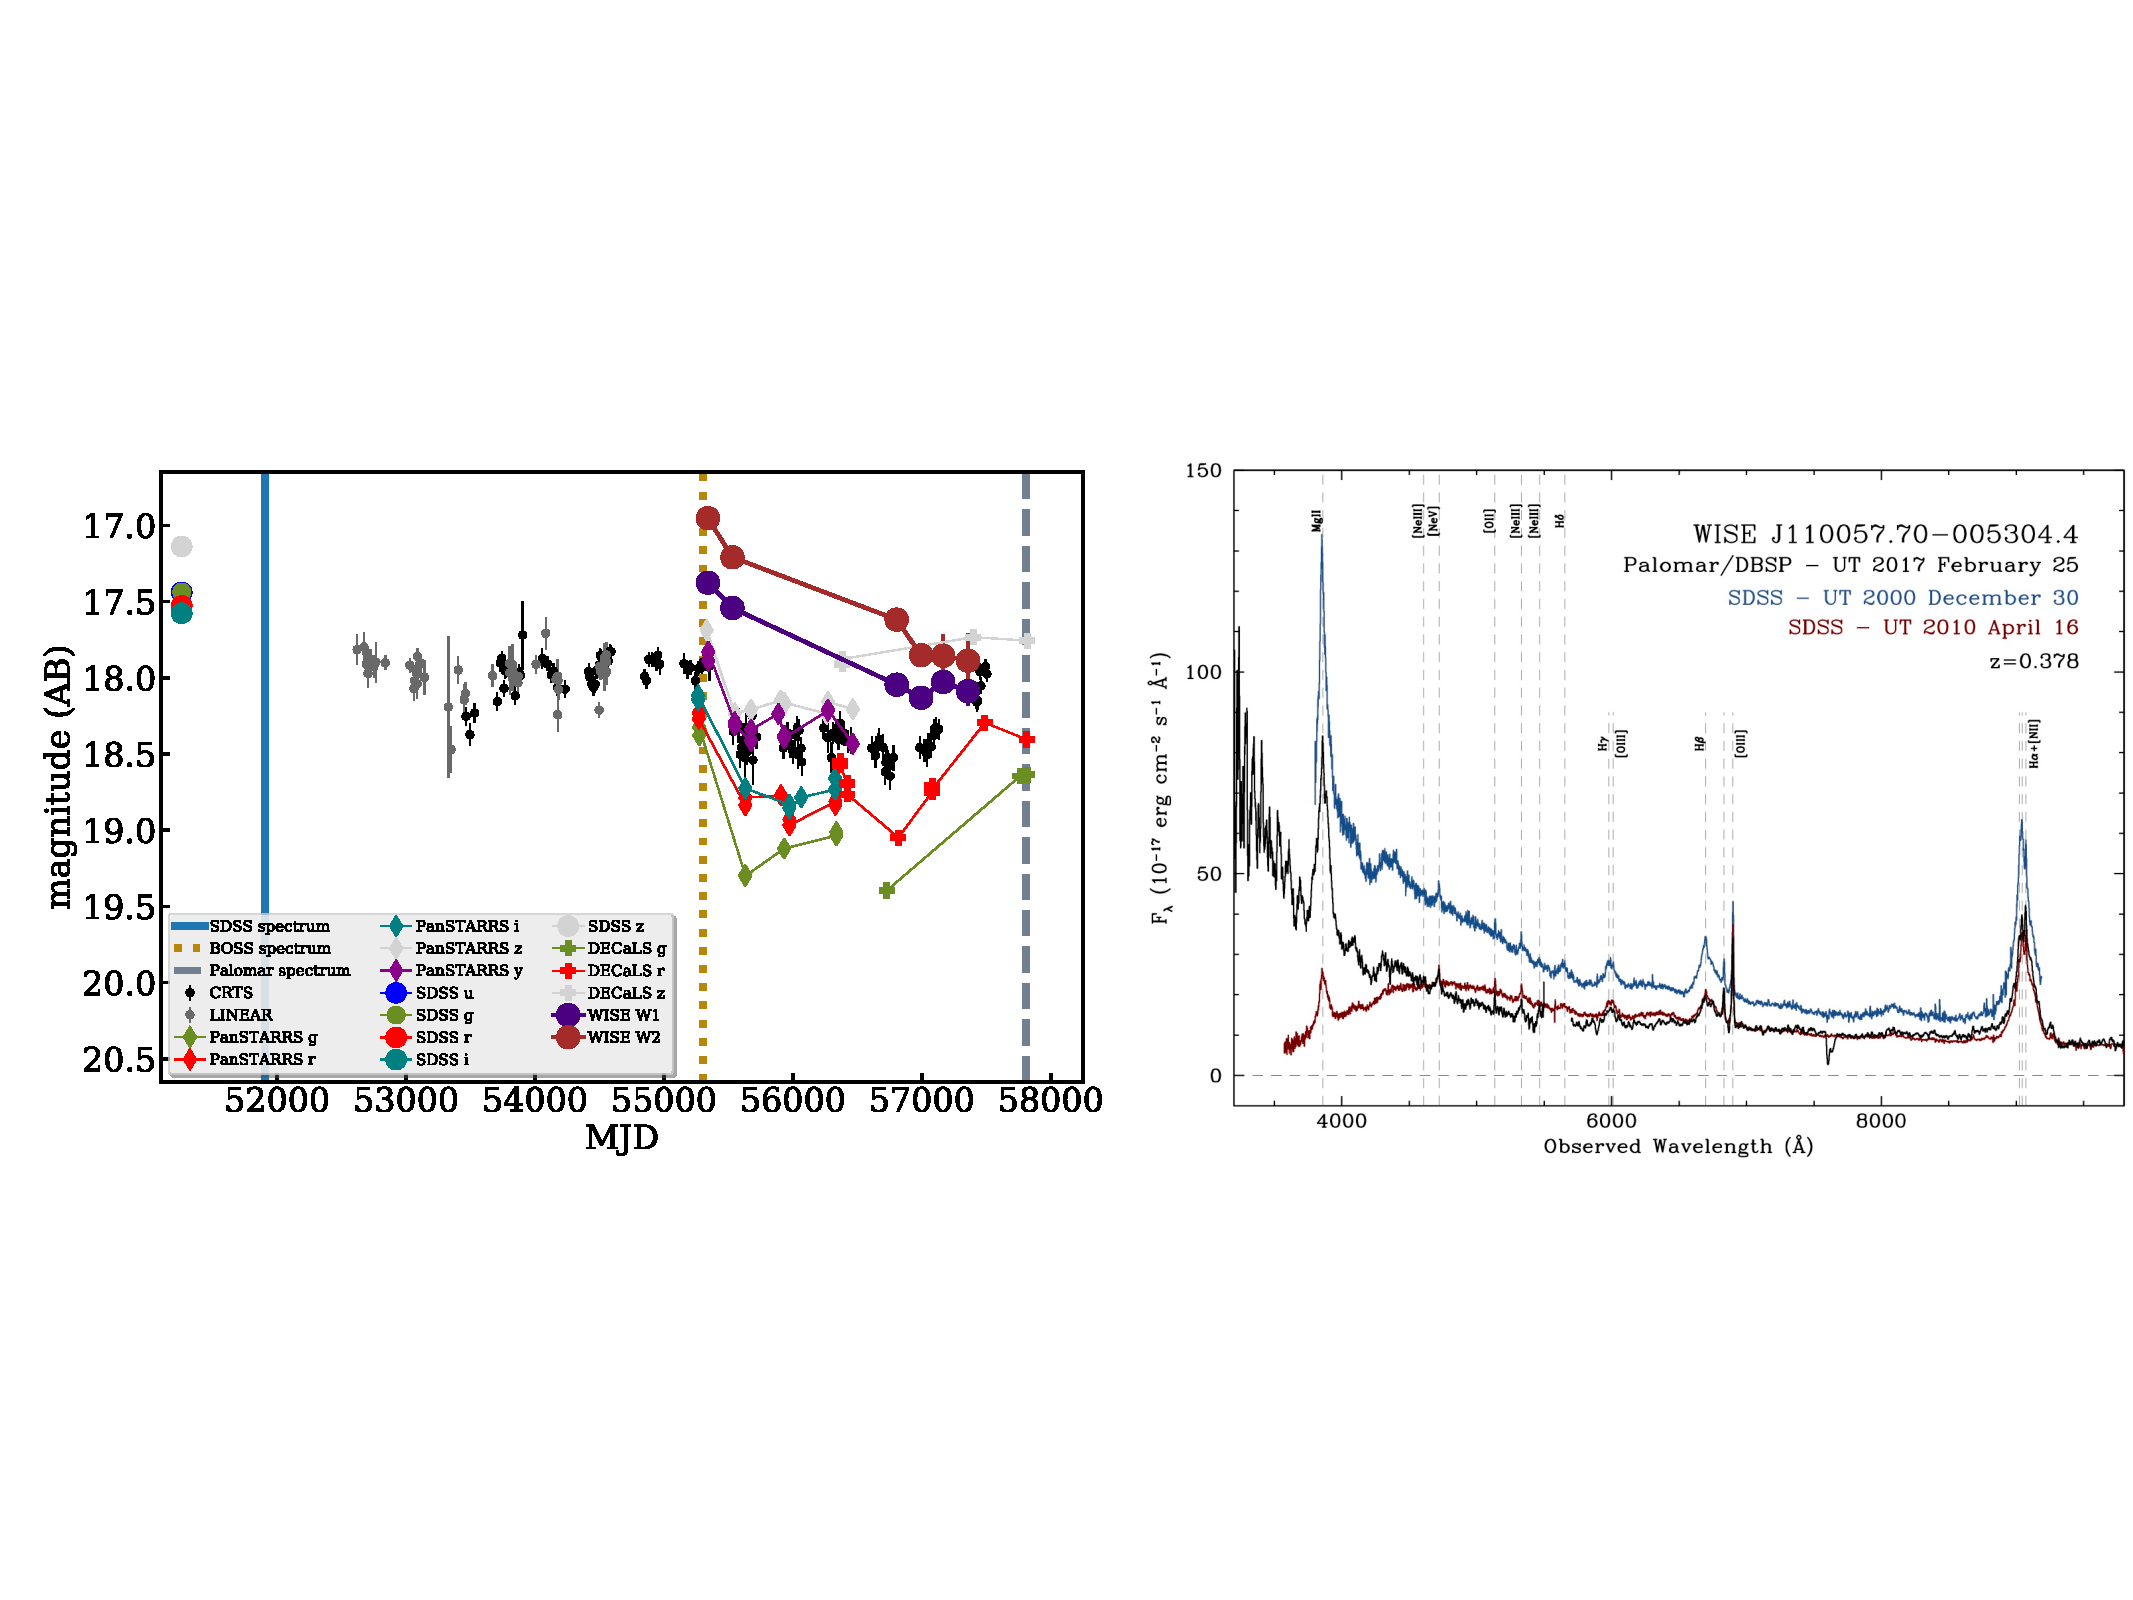
\includegraphics[height=6.25cm,width=17.2cm]
    {figures/J110057_LC_Spectra_20171024.pdf}
    \vspace{-10pt}
    \caption{%\small      
      \footnotesize 
      % \scriptsize
      % \tiny
      {\it (Left:)} The optical and infrared light-curve for the redshift $z=0.378$ quasar 
      J1100-0053 (Ross et al. 2018). 
      Note the fall in the infrared, whereas there is a decrease, but 
      then recovery in the optical. 
      {\it (Right:)} 
      Three epochs of spectra for J1100-0053. 
      The spectacular downturn in the blue for the 2010 spectrum 
      indicates a dramatic change in the accretion disk.
    }
  \vspace{-16pt}
 \label{fig:J110057}
\end{center}
\end{figure}


\smallskip
\smallskip
\noindent
During its initial phases of operation the Sloan Digital Sky
Survey (SDSS) obtained spectra of 1 million galaxies in the local
Universe. This dataset has become the {\it de facto} standard for
understanding the present day galaxy population, and sets the boundary
conditions for all theoretical comparisons. The paradigm changing
success of the SDSS was due to it having 1,000,000 objects {\it with very 
high SNR photometry and spectra}, enabling
multivariate analysis that is required for galaxy
astrophysics investigations.  {\it We desire the same sample size and revolutionary
understanding of the quasar population as the SDSS had with the
$z\sim0.1$ galaxy population.}  Our proposal takes quasar astrophysics
into the 2020s, going from single objects samples, to surveys and
samples of millions of objects, {\it with massive spectroscopic monitoring 
giving access to the time-domain} and leveraging these very large scale next
generation missions, telescopes and their datasets.




\begin{figure}[h]
  \begin{center}
   \hspace{-0.5cm}
%   trim=l b r t
    \includegraphics[width=16.0cm] %, trim={0.05cm 0 0.05cm 0},clip]
    {figures/Timelines_and_Facilites.pdf}
    \vspace{-10pt}
   \caption{Facilites, Timelines and Priorities. Withe SDSS and DESI in the Northern Hemisphere and 
4MOST, LSST in the South, we have full celestrial sphere coverage.}
  \vspace{-12pt}
 \label{fig:Keynote_facilites}
\end{center}
\end{figure}

\smallskip
\smallskip
\noindent
{\it The timing for this proposal could not be better.}  The first of
the data ``firehoses'' turns on in late 2019, with the full datastream
from our key sources fully online around 2022.  As such, we have the
time to mature our analysis techniques, and then being in the ideal
position to take advantage of the initial data releases of all these
new projects.

\smallskip
\smallskip
\noindent
The importance of this branch of astrophysics is already well
establish in Europe and is a priority for the next two decades. This
is demonstrated by noting that one of the two primary mission goals
for the Advanced Telescope for High-ENergy Astrophysics (ATHENA) mission 
is answering the question ``How do black holes grow and shape the
Universe?''.  ATHENA is ESA's second L-class flagship mission, due for
launch in 2028.


\smallskip
\smallskip
\noindent
{\it The scope and remit of an ERC Consolidator grant will allow us to
combine these data products in a manner that will not only establish
the new state-of-the-art in variable extragalactic astrophysics, it
will establish and kickstart the new field of variable extragalactic
astrophysics itself.}




\medskip
\medskip
\noindent
\large
{\bf{\textcolor{Cerulean}{2. Methodology}}}
\normalsize

\noindent
Our proposal contains eight work packages that fall into three broad and 
complementary categories: observational studies of large numbers
(millons) of objects; high-risk, very high-reward observational
studies of a small number (10s) of objects, and theoretical modeling
investigations. Risks and mitigation strategies are present for each
WP. Table 1 summarises our overal WP plan. 


\smallskip
\smallskip
\noindent
\textbf{\textsc{WP1: Build an Event Broker:}} 
The LSST will deliver three levels of data products and
services and being in the U.K. gives us access to all three. 
%The ``Level 3'' Data Products are the user-created data product services that will enable our science case. 
 In order to utilize the LSST data for our science needs we will need to build an {\it event
broker}, an intermediary program module that interacts with primarily
the ``Level 3'' data products from the LSST.
%% \noindent
{\bf WP1 is low-risk, high-reward.} 
The goal of this WP is to build an Event Broker.  The heavy-industry
computing infrastructure is already being supplied by the LSST Data
Access Center. Our task will be to build software in a timely and
robust manner. At the effort level of one PDRA (``PDRA 1'') and
commitment from the P.I., (NPR) along with the algorithm resources 
and key personel, e.g. Prof Andy Lawrence (AL) and Prof. Bob Mann (RGM),  
at the Royal Observatory, Edinburgh, there is no
element of this which can be deemed high-risk.


\smallskip
\smallskip
\noindent
\textbf{\textsc{WP2: Quasar Catalogue Generation:}} 
Building the quasar corpus and cataloguing the observational data will
be a large, but vital step in beginning to pursue our science
goals. This catalogue will be the glue that binds the observational
projects together and will have not only the data, but moreover the
metadata to enable the other WPs.
% \noindent
{\bf WP2 is low-risk, high-reward.}
The goal of this WP is to construct a quasar catalogue.
This is a full WP, and with the P.I.s (NPR) experience at this
specific task, plus the effort level of one PDRA (``PDRA 2'') there is
no element of this which can be deemed high-risk.


\smallskip
\smallskip
\noindent
\textbf{\textsc{WP3: Light-Curve and Spectral Analyses:}} 
Following on from the quasar corpus catalogue generation, one key
science output will be the full and detailed light-curve and spectral
analyses of the said catalogue. This will result in the discovery of
light-curve trends with quasar type, new methods to measure black hole
mass and the relatively easy check to see which quasars have become
``changing-look'' objects. This WP will have a data science/machine learning 
aspect.
% \noindent
{\bf WP3 is low-risk, high-reward.} 
The goal of this WP is to elucidate the physical processes that drive quasar variability.
The full Light-Curve and Spectral
Analyses that we envisaged will be a significant amount of work,
leading to significant high-reward science. This particular work
package will be broken down into small projects and the level of two
PDRAs (``PDRA 1'' and ``PDRA 2''), as well as the P.I. (NPR) and a PhD
student (``PhD 1'') will be directed towards this. This level of investigation 
is highly novel, but there is no element of this which can be deemed high-risk.


\smallskip
\smallskip
\noindent
\textbf{\textsc{WP4: Quasar Demographic studies:}} 
Another major scientific output that will originate from the quasar
corpus catalogue generation will be the study of the Quasar
Demographics from our datastreams. This is different from WP3 in that
these investigations wont necessarily be tied to the time-domain
aspect of our catalogue, but will be the crucial baseline that we, and
the field in general, will use to compare to the time-depedent
discoveries. Luminosity function, clustering and higher-order
statistics will be made in order to precisely determine the census of
AGN, their environments, their host galaxy preferences and their
evolution. All these are vital observational tests for galaxy
formation models and theory (see WP6 below).
% \noindent
{\bf WP4 is low-risk, high-reward.}
The goal of this WP is to make the key observational tests that have
to be explained by any viable galaxy formation theory.  Similar to
WP3, the analyses that we envisaged will be broken down into smaller
projects and the level of two PDRAs (``PDRA 1'' and ``PDRA 2''), as
well as the P.I. (NPR) and a PhD student (``PhD 1'') will be directed
towards this. There is no element of this which can be deemed
high-risk.


\smallskip
\smallskip
\noindent
\textbf{\textsc{WP5: Accretion Disk Simulation:}} 
New accretion models are needed to fully explain the observational
data of ``changing look'' quasars that we have examples of today (see
e.g. Ross et al. 2018). New radiation MHD codes begin to explain the
observations here, but further development is needed to gain the
desired deep understanding. 
% \noindent
{\bf WP5 is lower-risk, very high-reward.}
The goal of WP5 is to develop new accretion disk simulations that
explain our observational results.  This will be the lead WP for one
PDRA (``PDRA 3'') and a low level of the P.I.'s (NPR) time. We
classify WP5 not as fully `low-risk', since we envisage some ramp-up
time to get our theoretical simulations to the level that will be required by 
our beyond-the-state-of-the-art dataset. However, we mitigate this risk
by invoking the collaboration with an accretion disk theorist
Prof. Ken Rice (WKMR) who is the Personal Chair of Computational
Astrophysics in the School of Physics and Astronomy here at the
University of Edinburgh. NPR and WKMR and PDRA3 would thus collaborate 
on this WP. 


\smallskip
\smallskip
\noindent
\textbf{\textsc{WP6: AGN Feedback Simulations:}} 
Cosmological-scale hydrodynamic simulations are now coming online. 
While we do not seek to lead or generate new versions of these, we do 
envisaged using their outputs in order to `benchmark' our observational 
demographic work. 
% \noindent
{\bf WP6 is low-risk, high-reward.}
All the data from these simulations is already in place today, though no one 
has embarked on doing any of the `heavy-lifting' and comparisons we will 
have the observational results for. Professor Romeel Dave (RSD) who is a Chair of Physics 
in the Institute for Astronomy will be a key collaborator here. 
NPR and RSD and PDRA3 and/or PDRA2 would thus collaborate on this WP. 


\smallskip
\smallskip
\noindent
\textbf{\textsc{WP7: Observations of Quasars by the James Webb Space Telescope:}} 
What are the star-formation properties of mid-infrared luminous quasars at the peak of quasar activity? 
We aim to answer this by looking for the presence of polycyclic aromatic hydrocarbon (PAH) spectral features 
in $z \approx 2.5$ infrared bright quasars with the James Webb Space Telescope (JWST). 
% \noindent
{\bf WP7 is high risk, high-reward.}
This is an ideal investigation for the JWST, but we classify this as
`high-risk' since this is the one telescope/survey/mission where we
would have to bid and apply for the telescope time and are not guaranteed
the data. We mitigate the risk here by saying that this will be the
one project the P.I. (NPR) would directly lead, does not impact in any direct way any of
the other WPs and would lead to very-high gain science.


\smallskip
\smallskip
\noindent
\textbf{\textsc{WP8: New Object Discovery:}} 
The LSST will scan the sky repeatedly, enabling it, and us, to both
discover new, distant transient events and to study variable objects
throughout our universe. The most interesting science to come may well
be the discovery of new classes of objects.
% \noindent
{\bf WP8 is medium-to-high risk, exceptionally high-reward.}
We class this as medium-to-high risk, since it is tricky to class a WP
with essentially unknown discovery potential as fully `low-risk'.
Suffice to say, this would be exceptionally high-reward



\begin{figure}[h]
  \begin{center}
   \hspace{-0.5cm}
%   trim=l b r t
    \includegraphics[width=16.0cm] %, trim={0.05cm 0 0.05cm 0},clip]
    {figures/workplan.pdf}
    \vspace{-10pt}
 %  \caption{}
  \vspace{-12pt}
 \label{fig:Keynote_facilites}
\end{center}
\end{figure}


\smallskip
\smallskip
\noindent
\large
{\bf{\textcolor{Cerulean}{3. Resources,  Survey `buy-in' and Budget}}}
\normalsize

\smallskip
\smallskip
\noindent
\textbf{\textsc{Personnel:}} 
We request the resources and support for 90\% of the time and effort
for the P.I. (100\% is not claimed just in case non-project
opportunities arise, e.g. guest lecturing).  We request the resources and support for 3 Postdoctoral
Research Associates (PDRAs), for a total of 10 PDRA year
equivalents. This will be broken down as a three year term for ``PDRA
1'', a three year term for ``PDRA 2'' and a 2+2 year term for ``PDRA
3''.  We request the resources and support for 1 UK/EU PhD
studentship.


\smallskip
\smallskip
\noindent
\textbf{\textsc{Survery Buy-in:}} 
We request support for the ``buy-in'' to two of the new surveys,
SDSS-V and DESI. The costs here are \$230,000 (\euro184,100) for
SDSS-V and \$250,000 (\euro200,100) for DESI.  We ask this support to
come from the ``additional funds that can be made available to cover
access to large facilities.''  We specficially request access to these
funds as it gives our project the ``Full House'' of telescopes and
data in the North and Southern Hemispheres (for complete coverage of
the celestial sphere) and delivers the early spectroscopy that will be
vital to train, test and build our data science and machine learning
codes and algorthims. {\it Buy-in here would place the P.I. and the
University of Edinburgh as the only group and place in the world to be involved
in SDSS-V, DESI, 4MOST, LSST and ESA {\it Euclid} and JWST}.


\smallskip
\smallskip
\noindent
\textbf{\textsc{Computing Requirements:}} 
With the availability of the facilites at an institute (e.g. IfA
Cullen), university
(e.g. \href{https://www.ed.ac.uk/information-services/research-support/research-computing/ecdf}{``Edinburgh
Compute and Data Facility''} and at a national
{\href{https://www.hartree.stfc.ac.uk/Pages/home.aspx}{(The Hartree
Centre)} level, the rate limiting factor will be how quickly and
efficiently we can deploy our codes, and analysis, i.e. person-power.
%The rate limiting factor, in the vast majority of endevours, is (a) data access and (b) development.


\smallskip
\smallskip
\noindent
\textbf{\textsc{Travel:}} 
We request support for travel for all 5 members of the group,
including repeat medium-term (i.e., few weeks) travel to the US and
ESO Chile to work with key collaborators at critical timings of the
First Light for the new telescopes.




\newpage
\begin{center}
\medskip
 \medskip
 {\large \bf References}
    \vspace{-10pt}
\end{center}
\begin{multicols}{2}[]
\noindent
%\footnotesize
%\scriptsize
%\tiny
\lbrack 1\rbrack Kormendy \& Ho, 2013, ARAA, 51, 511\\
\lbrack 2\rbrack Kormendy,  2016, ASSL, 418, 431\\
\lbrack 3\rbrack Alexander et al., 2012, NewAR, 56, 93\\
\lbrack 4\rbrack King \& Pounds, 2015, ARAA, 53, 115 \\
\lbrack 5\rbrack Heckman \& Best, 2014, ARAA, 52, 589\\
\lbrack 6\rbrack Naab \& Ostriker, 2017, ARAA, 55, 59 \\
\lbrack 7\rbrack Netzer, 2015, ARAA, 53,  365\\
\lbrack 8\rbrack Padovani, 2017, A\&ARv, 25, 2\\
%%
\lbrack  9\rbrack Ata et al., 2017, arXiv1705.06373v2\\
\lbrack10\rbrack Solsar et al., 2013, JCAP, 04, 026 \\
\lbrack11\rbrack Busca et al.,  2013, A\&A, 552, 96 \\
\lbrack12\rbrack Delubac et al.,  2015, A\&A, 574, 59 \\
\lbrack13\rbrack Bautista et al., 2017, A\&A, 603, 12 \\
\lbrack14\rbrack du Mas des Bourboux et al., 2017, arXiv1708.02225v3\\
\lbrack15\rbrack Font-Riber et al., 2014, JCAP, 05, 027\\
%%
\lbrack16\rbrack Ross et al. 2015, MNRAS, 453, 3932\\
\lbrack17\rbrack Wright et al., 2010, AJ, 140, 1868\\
\lbrack18\rbrack Zakamska et al., 2016, MNRAS, 459, 3144\\
\lbrack19\rbrack Hamann et al., 2017, MNRAS, 464, 3431\\
%%
\lbrack20\rbrack Timlin, Ross et al., 2016, ApJS, 225, 1\\
\lbrack21\rbrack Timlin, Ross et al., 2017, ApJ, {\it in prep.}\\
%%
\lbrack22\rbrack LaMassa et al., 2015, ApJ, 800, 144\\
\lbrack23\rbrack Runnoe et al., 2016, MNRAS, 455, 1691\\
\lbrack24\rbrack Ruan et al, 2016, ApJ, 826, 188\\
\lbrack25\rbrack MacLeod, Ross et al., 2016, MNRAS, 457, 389\\
%%
\lbrack26\rbrack Meisner et al., 2017, AJ, 153, 38 \\
\lbrack27\rbrack Meisner et al., 2017, AJ, 154, 161 \\
% Meisner  et al., 2017, arXiv1710.02526v1 \\
\lbrack28\rbrack Ross et al., 2017, Nat.As., {\it in prep.} \\
%%
\lbrack29\rbrack Hopkins et al., 2006, ApJS, 163, 1\\
%%
\lbrack30\rbrack Schlegel et al., 2011,  arXiv:1106.1706v2 \\
%
\lbrack31\rbrack Ross et al., 2009, ApJ, 697, 1634 \\
%%
\lbrack32\rbrack Lombriser \& Taylor, 2016, JCAP, 03, 031 \\
\lbrack33\rbrack Baker et al, 2017,  arXiv1710.06394v1 \\
%%
\lbrack34\rbrack Watson et al.,  2011, ApJ, 740, L49\\
\lbrack35\rbrack King et al., 2014, MNRAS, 441, 3454\\
\lbrack36\rbrack King et al., 2015, MNRAS, 453, 1701\\
\lbrack37\rbrack Shen et al., 2015, ApJS, 216, 4\\
%\lbrack37\rbrack The Pierre Auger Collaboration, 2017, Science, 357, 6357 \\
\lbrack38\rbrack Hviding et al.,  2017, arXiv1711.01269v1 



\end{multicols}



\end{document}
